\documentclass[11pt]{article} 
\usepackage{xcolor} % Colors! 
\usepackage{listings} % For displaying code
\usepackage{float} % So figures stay where they should
\usepackage{graphicx} % Allows inclusion of graphics
\usepackage[font=small]{subcaption} % Caption font size adjustments
\usepackage[font=small]{caption} % " " 
\usepackage{multicol} % mulitple columns
\usepackage{hyperref} % for hyperlinks to websites/PDF index
\usepackage[margin=1in]{geometry} % Changes margins. 
\usepackage{kmap} % Karnaugh maps
\newcommand{\lstsetLaTeX}{%
\lstset{%
    language=TeX, % Change the listings language
    % frame=single, % Uncomment to show frame
    breaklines=true, % So the words don't run off the page
    postbreak=\raisebox{0ex}[0ex][0ex]{\ensuremath{\color{gray}\hookrightarrow\space}}, % Tab and cute arrow after a break
    commentstyle=\color{gray}    % comment style
}
}
\lstsetLaTeX

\setlength{\parindent}{0in} % Removes indentations
\setlength{\parskip}{6pt} % Adds space between paragraphs


\begin{document}
\vspace*{2.5cm} 

\begin{center}
    \LARGE
    \textbf{\LaTeX\ Tutorial}\\ 

    \medskip

    \large
    By Stephanie Soldavini and Andrew Ramsey 
\end{center}
\vfill

\copyright\ 2016 by Stephanie Soldavini and Andrew Ramsey. This work is licensed under the Creative Commons Attribution-ShareAlike 4.0 International License. To view a copy of this license, visit \url{http://creativecommons.org/licenses/by-sa/4.0/}.

Please send feedback to \href{mailto:axr8451@rit.edu}{\nolinkurl{axr8451@rit.edu}}

\newpage


\section*{What is \LaTeX\ and why it should be used}
\addcontentsline{toc}{section}{What is \LaTeX\ and why it should be used}
\LaTeX\ is a computer program that allows the production of professional looking papers with minimal effort, after a bit of a learning curve. It allows for the use of templates in a much more straightforward manner than Word, which makes it the typesetting program of choice in many professional journals. For this reason, knowing \LaTeX\ will make writing technical reports much easier, as the general format will not change.


\section*{Setup}
\addcontentsline{toc}{section}{Setup} % This adds the starred section to the table of contents
\begin{itemize} 
    \item Windows - Go to \url{http://miktex.org/download} and select the appropriate 32 or 64 bit version (64 bit will need to expand "Other Downloads"). Launch it and follow the instructions.

    \item Mac - Go to \url{http://www.tug.org/mactex/mactex-download.html} and select the pkg file. Run that and follow the instructions. 

    \item Linux - Use the package manager to install. The package will be different depending on the distro. Generally installing "texlive" will be enough, but in some cases, there will be other packages that provide additional functionality. 

    \item Other options - Should the above process be too much effort or the computer does not have enough space, there are online editors that will produce a PDF. Some can be found here. \url{https://en.wikibooks.org/wiki/LaTeX/Installation#Online_solutions} 


\end{itemize}
        Should any issues arise, check \url{https://en.wikibooks.org/wiki/LaTeX/Installation}. This website also contains other useful information related to \LaTeX.

\subsection*{Editors}
\addcontentsline{toc}{subsection}{Editors}
Any plain text editor will do, but some are certainly easier than others. A list is available here: \url{https://en.wikibooks.org/wiki/LaTeX/Installation#Editors}. Vim or Emacs can be used as well, and have plugins available for \LaTeX\ to make things simpler.

\section*{General format}
\addcontentsline{toc}{section}{General format}
\begin{lstlisting}
\documentclass[11pt]{article} % This must be the first line. It declares the type of document and the font size.

% Below is the "preamble." This is where usepackages and other declarations that affect the body go.

\usepackage[margin=1in]{geometry} % Changes margins. Default LaTeX margins are ridiculous. 
\usepackage{graphicx} % Allows inclusion of graphics
\usepackage{amsmath} % Math symbols
% Other packages go here

\begin{document} % This is what starts the body of the document 
    
    Text and code go here!

    A blank line or "\\" need to be between sections that should be separate paragraphs. 
    Two lines like 
    this will output as a single line. 

\end{document} % This ends the document. Don't forget this or the document won't compile.
\end{lstlisting}

\section*{Headers}
\addcontentsline{toc}{section}{Headers}
To make a header, use the command: 

\begin{lstlisting}
\section*{Header Title Here}
\end{lstlisting}

The \texttt{*} removes the section numbers. If section numbers are desired (and they are not in this class), use: 

\begin{lstlisting}
\section{Header Title Here}
\end{lstlisting}

\subsection*{Subsections}
\addcontentsline{toc}{subsection}{Subsection}

For subsections like above, use the following:

\begin{lstlisting}
\subsection*{Subsection}
\end{lstlisting}

Generally this will not be necessary for this class. 

\subsubsection*{Subsubsections}
\addcontentsline{toc}{subsubsection}{Subsubsection}

For an even lower level header, use the following: 

\begin{lstlisting}
\subsubsection*{Subsubsections}
\end{lstlisting}

\section*{Tables}
\addcontentsline{toc}{section}{Tables}

The standard table format is as follows:

\begin{lstlisting}
\begin{table}[H] % H makes it stay in place (needs float package)
    \centering % centers the table 
    \caption{Put the descriptive table caption here}
    \label{tab:MyAwesomeTableLabel}
    \begin{tabular}{lcr} % "lcr" describes alignment of each column 
        Col 1 & Col 2 & Col 3 \\ \hline % "\hline" adds horizontal line
        Hello & This is a cell & Tableee \\ % "\\" after each row
        Wheee & Very imporant information lives here & Yes \\
        Row 3 & Row 3 & Row 3 \\ 
    \end{tabular}
\end{table}
\end{lstlisting}

This code yields: 
\begin{table}[H]
    \centering
    \caption{Put the descriptive table caption here}
    \label{tab:MyAwesomeTableLabel}
    \begin{tabular}{lcr}
        Col 1 & Col 2 & Col 3 \\ \hline
        Hello & This is a cell & Tableee \\
        Wheee & Very imporant information lives here & Yes \\
        Row 3 & Row 3 & Row 3 \\ 
    \end{tabular}
\end{table}


\subsection*{Table column alignment}
\addcontentsline{toc}{subsection}{Table column alignment}

In the above example ``lcr'' is used. This means that the first column is left-aligned, the second column is centered, and the third column is right-aligned. 

Pipe symbols (\textbar ) can be used to add vertical lines. ``l\textbar c\textbar\textbar ll'' would make a table where the first and second columns are separated by a sinlge vertical line and the second and third columns are separated by a double vertical line. The third and fourth columns are not separated by a line. 

\section*{Images}
\addcontentsline{toc}{section}{Images}


The standard image format is:

\begin{lstlisting}
\begin{figure}[H] % Don't forget the float package!
    \centering
    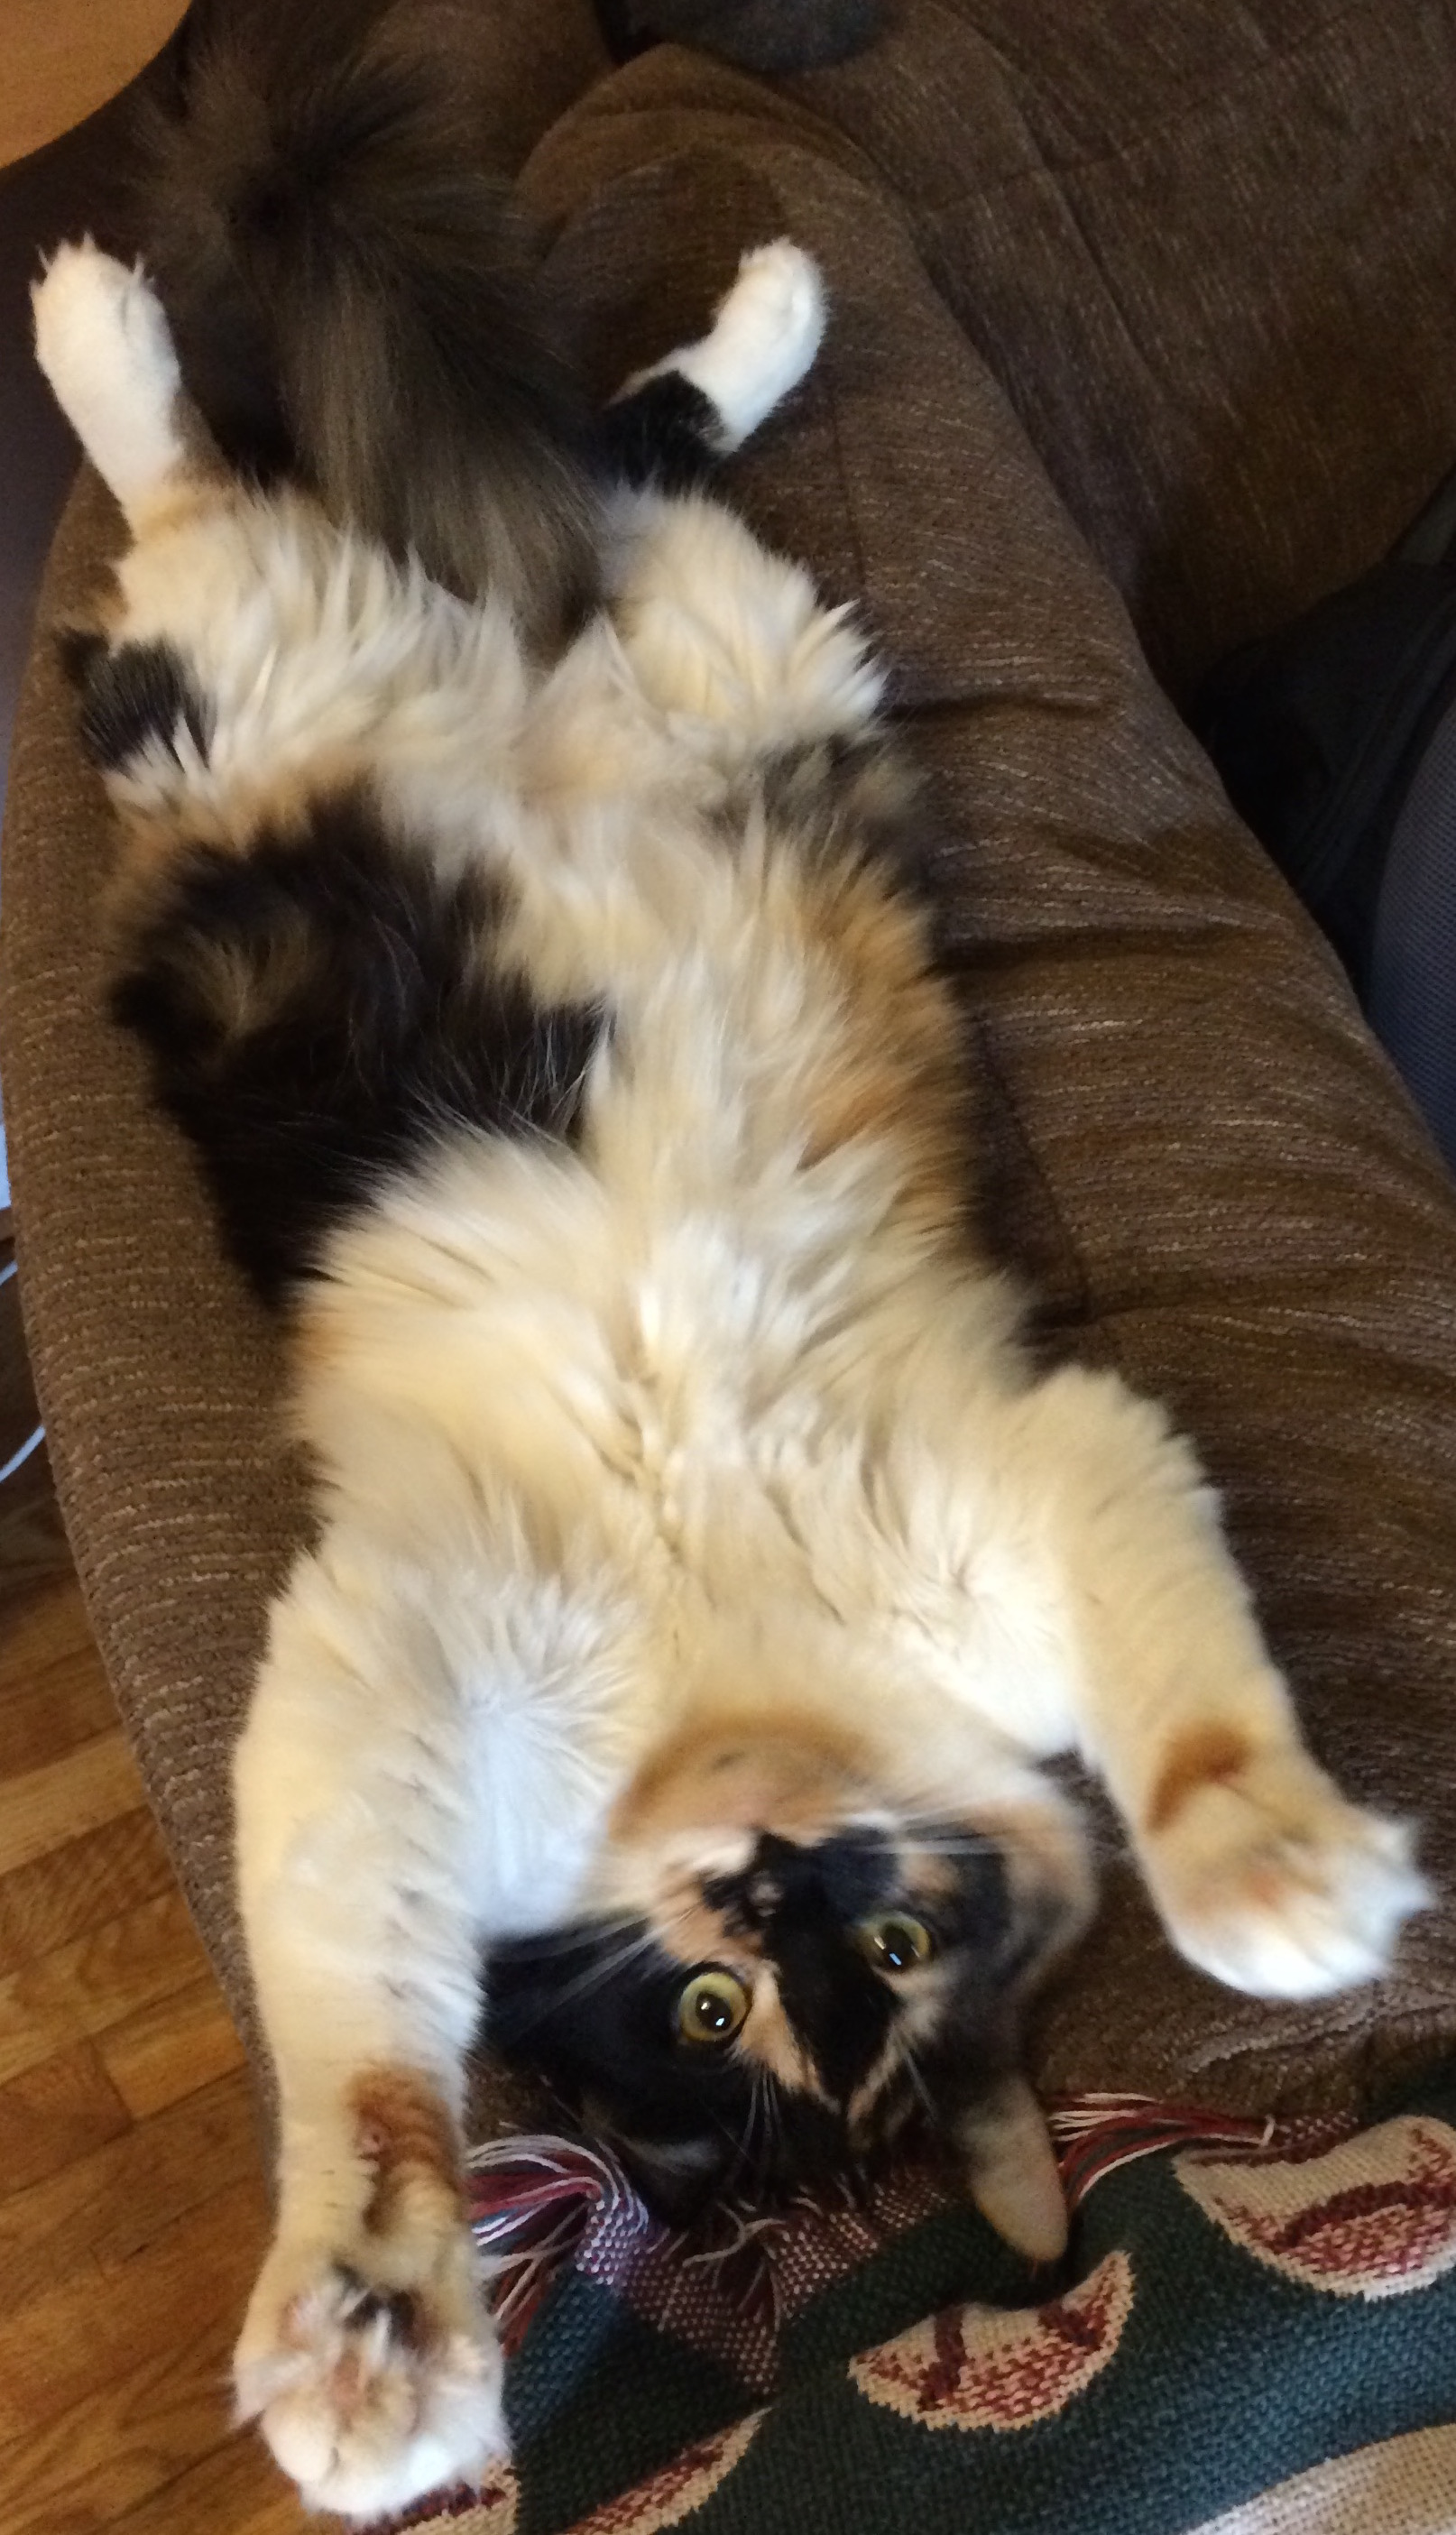
\includegraphics[width=.35\textwidth]{mycatCrookshanks} % no extension necessary
    \caption{This is my nerd cat, Crookshanks.}
    \label{fig:myAwesomeImageLabel}
\end{figure}
\end{lstlisting}

\newpage

This code yields:
\begin{figure}[H] % Don't forget the float package!
    \centering
    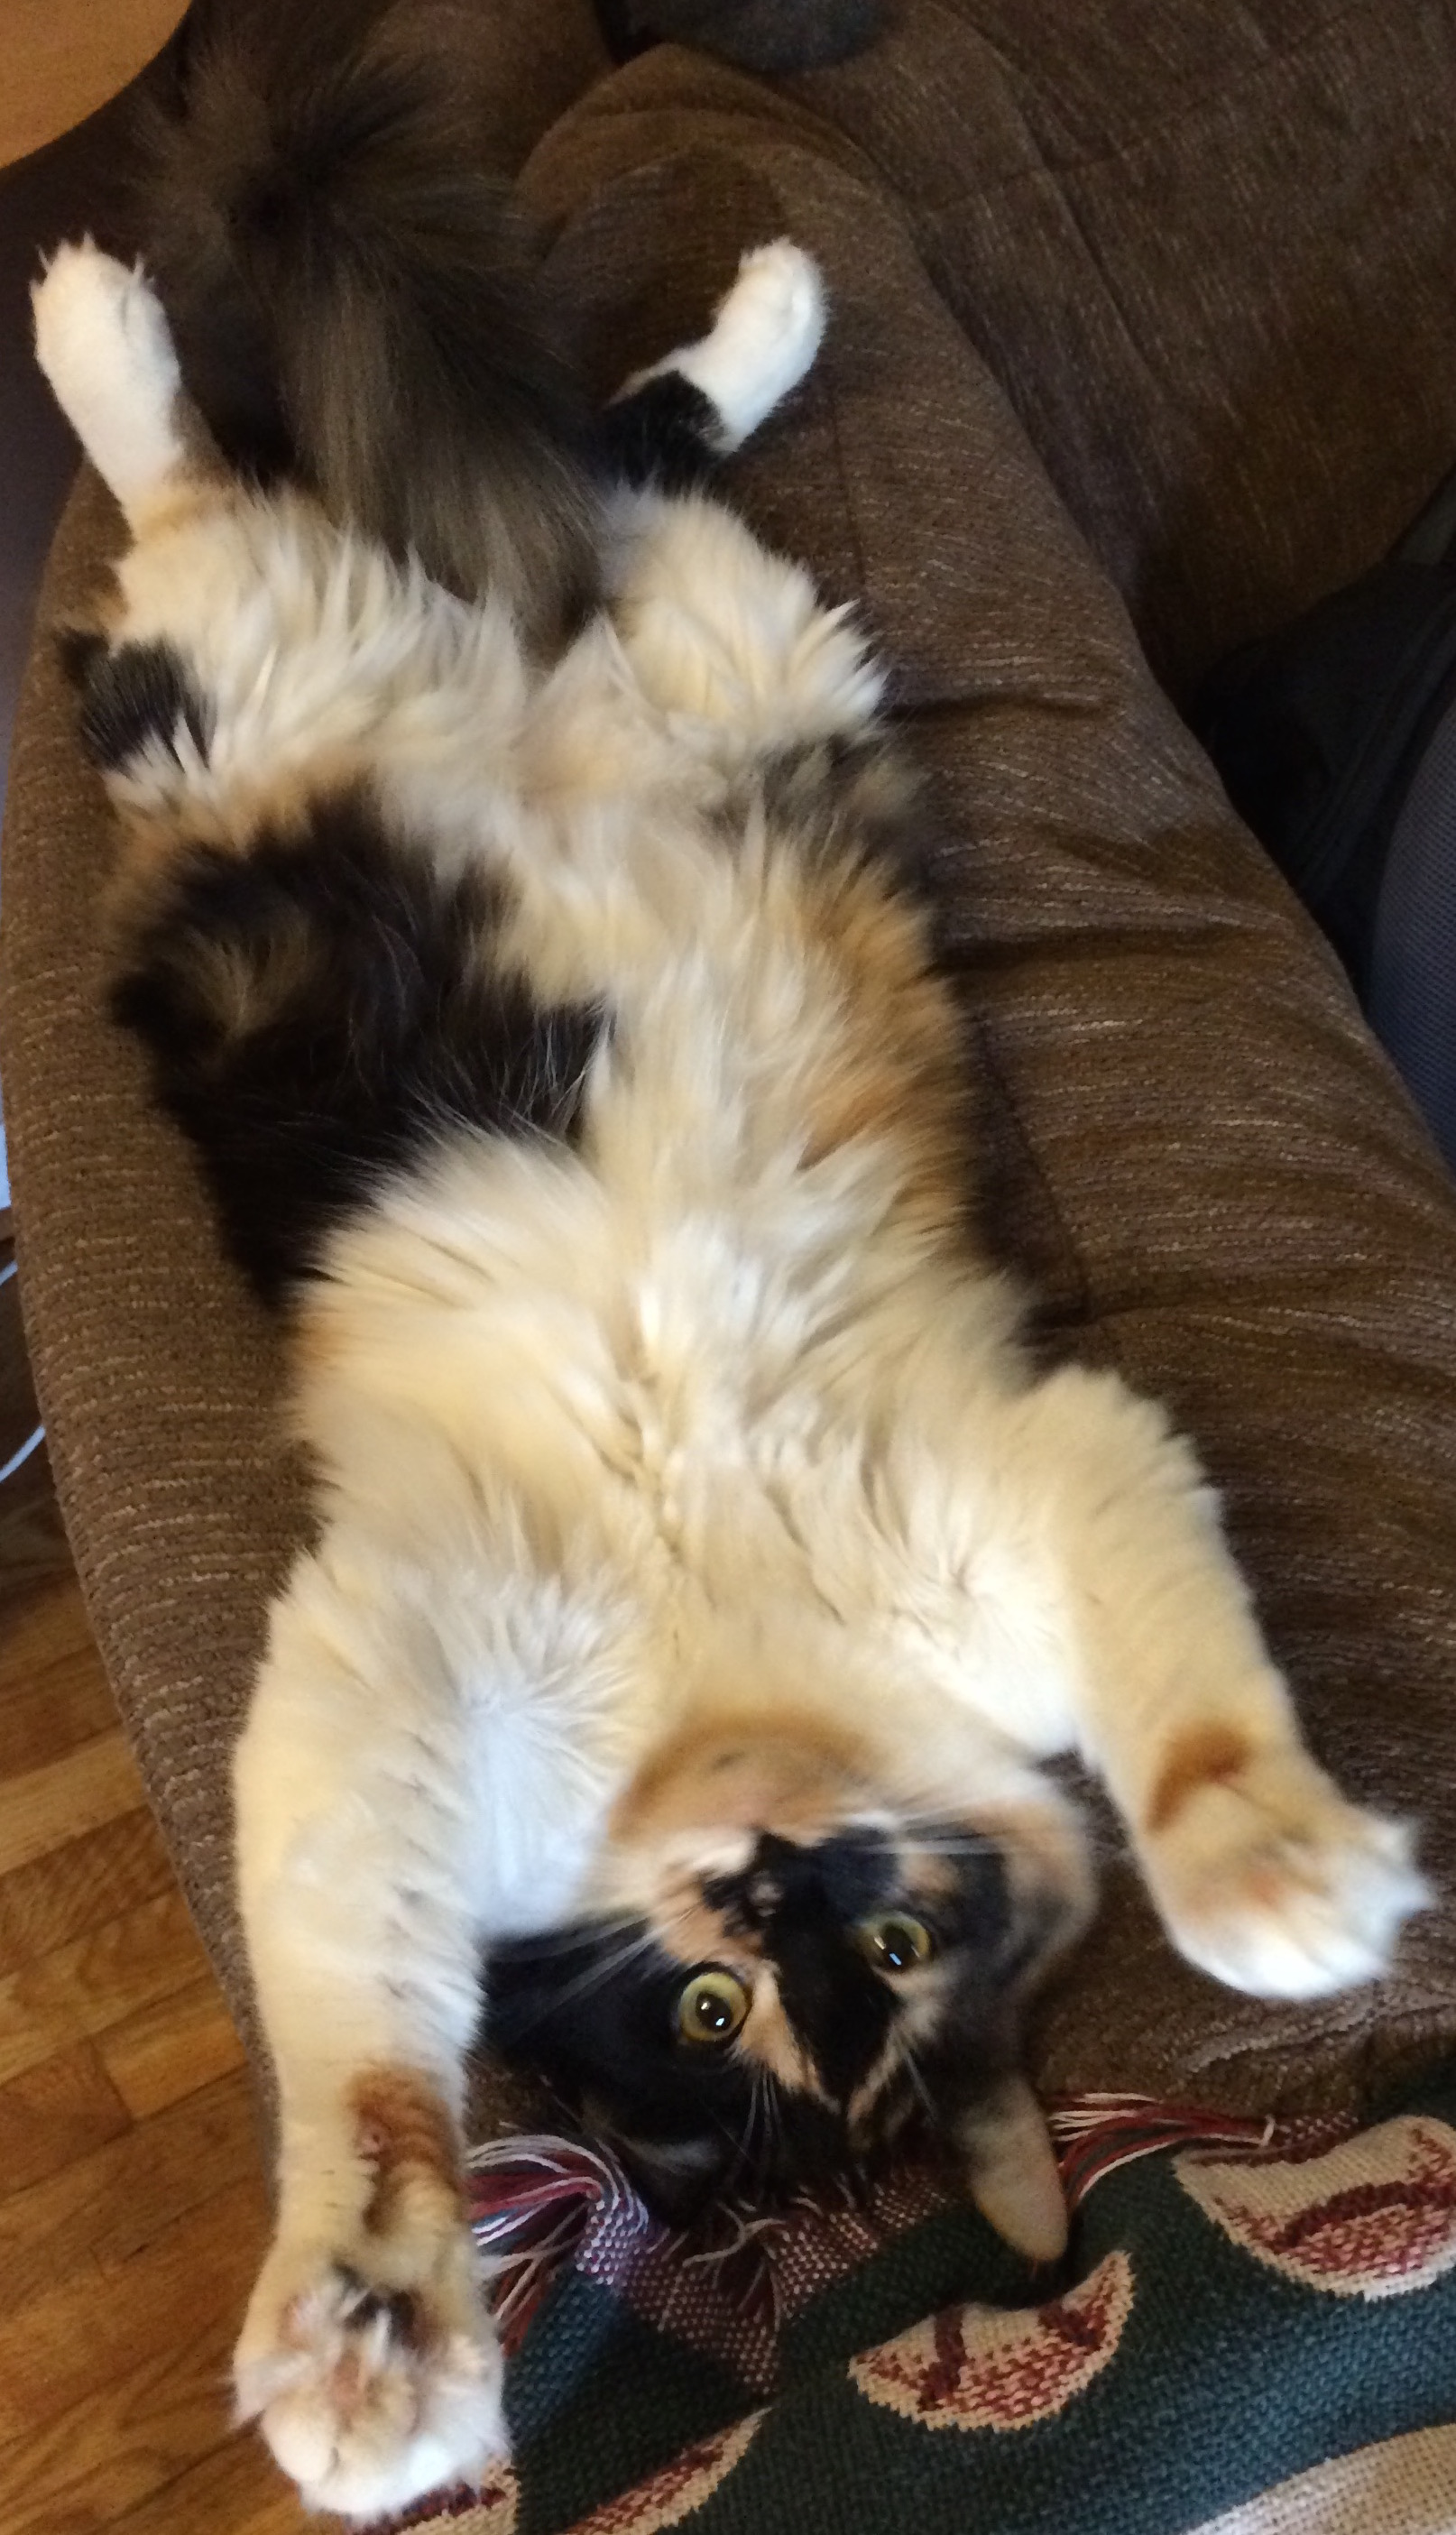
\includegraphics[width=.35\textwidth]{mycatCrookshanks} % no extension necessary
    \caption{This is my nerd cat, Crookshanks.}
    \label{fig:myAwesomeImageLabel}
\end{figure}

\subsection*{Image sizing}
\addcontentsline{toc}{subsection}{Image sizing}
\LaTeX\ will automatically insert the image in a 1:1 ratio with the size if no other instructions are given. In the example above, the image is 0.35x the width of the text, as specified by \\ \texttt{width=0.35$\backslash$textwidth}. Omitting the 0.35 will cause the image to take up the whole text width. Note that textwidth does not change with the use of environments such as itemize, but other options such as linewidth do. Specific sizes such as \texttt{width=4in} can also be used. 

\section*{Equations}
\addcontentsline{toc}{section}{Equations}
The standard equation format is as follows:

\begin{lstlisting}
\begin{equation}
    \overline{A + B} = \overline{A}\,\overline{B}
    \label{eq:SuperEQ}
\end{equation}
\end{lstlisting}

This code yields:
\begin{equation}
    \overline{A + B} = \overline{A}\,\overline{B}
    \label{eq:SuperEQ}
\end{equation}

\LaTeX\ supports much more in equation environments than is reasonable to cover. A few things to know:
\begin{itemize}
    \item Whitespace is ignored. Spacing is controlled by a "\textbackslash" followed by a semicolon, colon, or comma, depending on the spacing desired. Semicolons provide the most space, and commas the least. Exclamation marks produce negative space.
    \item For an inline environment, use dollar signs. For example writing $F_{SOP}$, is done by writing \verb|$F_{SOP}$|. The braces around \texttt{SOP} ensure that all three letters are subscript, not just the first one, like so: $F_SOP$. This equation is not counted in the numbering. 
    \item Non-numbered, centered equations can be produced with the \texttt{equation*} environment provided by the amsmath package.
        \item Multiple centered equations are best written with the \texttt{align} environment, from the amsmath package. More information is available at \url{https://en.wikibooks.org/wiki/LaTeX/Advanced_Mathematics#align_and_align.2A}.
\end{itemize}

\section*{References}
\addcontentsline{toc}{section}{References}
Having created a figure, table, or equation, it is useful to be able to refer to it in text, either before or after it appears. For example, putting \verb|Table~\ref{tab:MyAwesomeTableLabel}| would produce Table~\ref{tab:MyAwesomeTableLabel}. The tilde ensures that the number is not separated from the word. Because of the hyperref package, the number is clickable, though that is not necessary. The same \verb|\ref{}| command can be used for equations and figures. For example, \verb|Figure~\ref{fig:MyKMap}| produces Figure~\ref{fig:MyKMap}, even though that figure has not yet appeared. 

This is one of the major benefits of \LaTeX, as it means that rearranging figures will not require them to be renumbered, throwing off the references. \LaTeX takes care of this behind the scenes. 

\section*{Itemize/Enumerate}
\addcontentsline{toc}{section}{Itemize/Enumerate}

The itemize and enumerate environments are very similar, the primary difference being that itemize produces bulleted lists by default and enumerate numbered lists. The focus here will be on enumerate. The standard enumerate format is as follows:

\begin{lstlisting}
\begin{enumerate}
    \item The first item
    \item Another super cool item
    \item % Text could go here, pushing the nested onto a new line 
        \begin{enumerate} % It's good to indent this so it is obviously nested 
            \item Nested is useful
            \item More nesting could be done
        \end{enumerate}
\end{enumerate}
\end{lstlisting}

\newpage

This code yields: 

\begin{enumerate}
    \item The first item
    \item Another super cool item
    \item % Text could go here, which will push the nested numbers onto a new line 
        \begin{enumerate} % It's good to indent this so it is obviously nested 
            \item Nested is useful
            \item More nesting could be done
        \end{enumerate}
\end{enumerate}

\section*{Multiple columns}
\addcontentsline{toc}{section}{Multiple columns}
Generally, multiple columns should not be used. There are a few exceptions, primarily the cover sheet, which is already done, and for headers in tables. Say Table~\ref{tab:MyAwesomeTableLabel} should have a header that spans both column one and two. By using the multicol package, this would be possible. The code to do so looks like this: 
\begin{lstlisting}
\begin{table}[H] 
    \centering 
    \caption{A Cool Table with Multiple Columns}
    \label{tab:MyAwesomeMultiColTab}
    \begin{tabular}{lcr} % A multicolum command will span more than one column
        \multicolumn{2}{c}{Col 1 and 2} & \\ \cline{1-2} % cline is like hline but requires a column range
        Col 1 & Col 2 & Col 3 \\ \hline     
        Hello & This is a cell & Tableee \\ 
        Wheee & Very imporant information lives here & Yes \\
        Row 3 & Row 3 & Row 3 \\ 
    \end{tabular}
\end{table}
\end{lstlisting}

This code yields:


\begin{table}[H] 
    \centering 
    \caption{A Cool Table with Multiple Columns}
    \label{tab:MyAwesomeMultiColTab}
    \begin{tabular}{lcr} % A multicolum command will span more than one column
        \multicolumn{2}{c}{Col 1 and 2} & \\ \cline{1-2} % cline is like hline but requires a column range
        Col 1 & Col 2 & Col 3 \\ \hline     
        Hello & This is a cell & Tableee \\ 
        Wheee & Very imporant information lives here & Yes \\
        Row 3 & Row 3 & Row 3 \\ 
    \end{tabular}
\end{table}

Breaking down the \verb|\mutlicolumn{}{}{}| command more, it takes three arguments. The first is the number of columns it should span, the second is the alignment (left, right, or center) and the third is the text that should be displayed. Notice the there is only one ampersand in the row with this command. \LaTeX\ understands that it is taking up two columns and will not throw an error.

\section*{Special things}
\addcontentsline{toc}{section}{Special things}

\subsection*{Code}
\addcontentsline{toc}{subsection}{Code}
Sometimes it will be necessary to display code in the document, like this one. The listings package provides a convenient means to do so. The code to do so is as follows (Sadly \LaTeX\ does not allow for the easy nesting of lstlisting environments, so there's no syntax highlighting this time):

\begin{verbatim}
\lstset{language=Python}
\begin{lstlisting}
    print("Hello World") # My very first Python program
\end{lstlisting}
\end{verbatim}

This code yields: 
\lstset{language=Python}
\begin{lstlisting}
    print("Hello World") # My very first Python program
\end{lstlisting}

Notice that the \verb|\lstset{}| command caused the code to be interpreted as Python instead of \LaTeX. Without it the code would appears like this: 

\lstsetLaTeX
\begin{lstlisting}
    print("Hello World") # My very first Python program
\end{lstlisting}

\subsection*{K-Maps}
\addcontentsline{toc}{subsection}{K-Maps}
K-Maps are very useful when working with Boolean Algebra. A package exists that makes them much simpler to produce, but is not included with \LaTeX\ like the other packages have been. Instead the kmap.sty file must be placed in the same directory as the .tex file. \verb|\usepackage{kmap}| must be placed at the top of the file with the other \verb|\usepackage{}| commands. Don't forget that \verb|\usepackage{float}| is required to use \texttt{H} with \verb|\begin{figure}|.

The standard K-Map format is as follows: 
\begin{lstlisting}
\begin{figure}[H]
    \centering
    \begin{Karnaugh}[A][B][C][D]
        \contingut{0,1,0,0,1,0,1,1,0,1,0,0,0,0,1,1} % Put these in numerical order
        \implicantLateral[2pt]{4}{6}{green} % Wraps around the side and is slightly larger
    	\implicant{7}{14}{green} % Since the 2pt is in square brackets it is optional
    	\implicantTopBottom{1}{9}{red} % Different colors are possible
	\end{Karnaugh}
	\caption{A Nice Looking K-Map}
	\label{fig:MyKMap}
\end{figure}
\end{lstlisting}

\newpage 

This code yields:

\begin{figure}[H]
    \centering
    \begin{Karnaugh}[A][B][C][D]
        \contingut{0,1,0,0,1,0,1,1,0,1,0,0,0,0,1,1} % Put these in numerical order
        \implicantLateral[2pt]{4}{6}{green} % Wraps around the side and is slightly larger
    	\implicant{7}{14}{green} % Since the 2pt is in square brackets it is optional
    	\implicantTopBottom{1}{9}{red} % Different colors are possible
	\end{Karnaugh}
	\caption{A Nice Looking K-Map}
	\label{fig:MyKMap}
\end{figure}

The \verb|\implicant{}| command and its variations take 3 required arguments and one optional. The required arguments, in order, are the top left cell, the bottom right cell, and the filling color. The optional argument is the amount to add to the size of the group. Negatives are allowed. The exceptions to this rule are \verb|\implicantIso{}| which only requires one cell, and \verb|implicantCorners{}|, which takes no cell arguments. 

\subsubsection*{Possible modifications}
\addcontentsline{toc}{subsubsection}{Possible modifications}
A three variable version is also possible by exchanging \texttt{Karnaugh} for \texttt{Karnaugh3Var}. In this case, the contingut should only contain 8 values, instead of 16. The two variable K-Map, \texttt{Karnaugh2Var}, is another option.

\smallskip

To change the literals displayed on the K-Map, change the optional arguments \texttt{A}, \texttt{B},\texttt{C}, and \texttt{D} to the desired values. Note that mathmode is automatically implied, so writing \texttt{[S\_1]} will work, while \texttt{[\$S\_1\$]} will not.


\subsection*{State diagrams}
\addcontentsline{toc}{subsection}{State Diagrams}
No nice package for state diagram has been found, however, this website (\url{http://madebyevan.com/fsm/}) makes the creation of them straightforward. The site allows the exporting of \LaTeX\ code that can be copied and pasted into the document, though it will be necessary to wrap the code inside a figure environment, just as was done with the K-Map. It only requires the tikz package. 

\section*{Detexify}
\addcontentsline{toc}{section}{Detexify}
Some commands are hard to remember, but not to worry, Detexify knows them. It will produce few options based on what is drawn, as well as the packages and mode in which the command can be used. Try it at \url{http://detexify.kirelabs.org/classify.html}


\section*{Extra Commands}
\addcontentsline{toc}{section}{Extra Commands}
\begin{itemize}
    \item \verb|\newpage| - Starts a new page at that location. 
    \item \verb|\LARGE| - Changes the text size. Other options available at \url{https://en.wikibooks.org/wiki/LaTeX/Fonts#Sizing_text} 
    \item \verb|\medskip| - Produces vertical space at the point. See \url{https://en.wikibooks.org/wiki/LaTeX/Lengths#Fixed-length_spaces} for the other sizes.
    \item A lot more - \url{https://en.wikibooks.org/wiki/LaTeX/Command_Glossary} 
\end{itemize}
\section*{Some Final Notes}

Much of the formatting required for CMPE-160, for which this tutorial was written, has already been done. To make use of this, download the files from \url{https://github.com/DeepHorizons/KGCOEReport_template} and place them in the same directory as the tex file. Then, instead of \verb|\documentclass[11pt]{article}|, write \verb|\documentclass[CMPE]{KGCOEReport}|. This tells \LaTeX to import the formatting from the downloaded file.
\end{document}
